% !TEX TS-program = XeLaTeX
% !TEX spellcheck = en-US
\documentclass[aspectratio=169]{beamer}

\usetheme{example}

\title{Lecture 7:\\ Ensemble Methods}
\institute{GRA4160: Predictive modelling with machine learning}
\date{February 21st 2025}
\author{Vegard H\o ghaug Larsen}

\begin{document}

\maketitle

\frame{
    \frametitle{Plan for today:}
    \begin{itemize}
        \item Introduction to ensemble methods
        \item Bagging
        \item Boosting
        \item Recap decision trees
        \item Random forests
        \item Extra trees
    \end{itemize}
}

\frame{
    \frametitle{Ensemble methods}
    \begin{itemize}
        \item A family of techniques that involve training multiple models and combining their predictions to form a more accurate and robust model
        \item Can be used with a variety of models (e.g. linear models, decision trees, or neural networks)
        \item By combining multiple models, the ensemble typically reduces variance and often boosts performance
        \item \textbf{A trade-off:} ensembles are often more powerful, but can be less interpretable than single models
        %COMMENT: Added note on interpretability trade-off and general statement on reducing variance for clarity.
    \end{itemize}
}

\frame{
    \frametitle{Types of Ensemble Methods}
    \begin{itemize}
        \item \textbf{Bagging} (Bootstrap Aggregating)
        \begin{itemize}
            \item Examples: Random Forests, Extra Trees
            \item Reduces variance by training multiple models on bootstrap samples and averaging predictions
        \end{itemize}
		\pause
        \item \textbf{Boosting} (Sequential Learning)
        \begin{itemize}
            \item Examples: Gradient Boosting, AdaBoost, XGBoost
            \item Trains models sequentially, focusing on misclassified examples to reduce bias
        \end{itemize}
		\pause
        \item \textbf{Bayesian Model Averaging} (BMA)
        \begin{itemize}
            \item Trains multiple models and assigns weights based on posterior probabilities
            \item Can dynamically update model weights as new data becomes available
            \item Useful when model uncertainty needs to be explicitly accounted for
        \end{itemize}
		\pause
        \item \textbf{Stacking} (Stacked Generalization)
        \begin{itemize}
            \item Combines multiple models by training a meta-model on their outputs
            \item Often uses diverse base models (e.g., decision trees, SVMs, neural networks) to leverage complementary strengths
            \item Example: A neural network trained on outputs of logistic regression, SVM, and a random forest
        \end{itemize}
        % COMMENT: Expanded descriptions, added advantages, examples, and use cases for clarity.
    \end{itemize}
}

\frame{
	\frametitle{Bagging}
	\begin{center}
		{\LARGE Bagging}
	\end{center}
}

\frame{
    \frametitle{Bagging}
    \begin{itemize}
        \item Bagging is short for \textbf{Bootstrap AGGregatING}
        \item Train multiple instances of a base model on \textit{bootstrap} samples of the training data
        \item Combine their predictions (via majority vote or averaging) to form a final prediction
        \item Subsets are created using sampling with replacement
        \item Effective at reducing variance and mitigating overfitting for high-variance base learners (e.g., large decision trees)
        \item An \textbf{out-of-bag (OOB) error} estimate can be obtained without a separate validation set
        %COMMENT: Added the mention of OOB error and expanded on how bagging can reduce overfitting.
    \end{itemize}
}

\begin{frame}{Bootstrap in Machine Learning}
\begin{itemize}
    \item A resampling technique to approximate the sampling distribution of a statistic
    \item Repeatedly sample with replacement to create new datasets of the same size as the original
    \item About 63\% of unique samples from the original dataset typically appear in each bootstrap sample
    \item Used to train multiple models (bagging) or provide performance estimates (e.g.\ OOB error)
    \item Especially useful for small datasets or when data is expensive to collect
    %COMMENT: Added the 63% fact and a note on small datasets for clarity.
\end{itemize}
\end{frame}

\begin{frame}{Bootstrap sampling}
	\begin{center}
		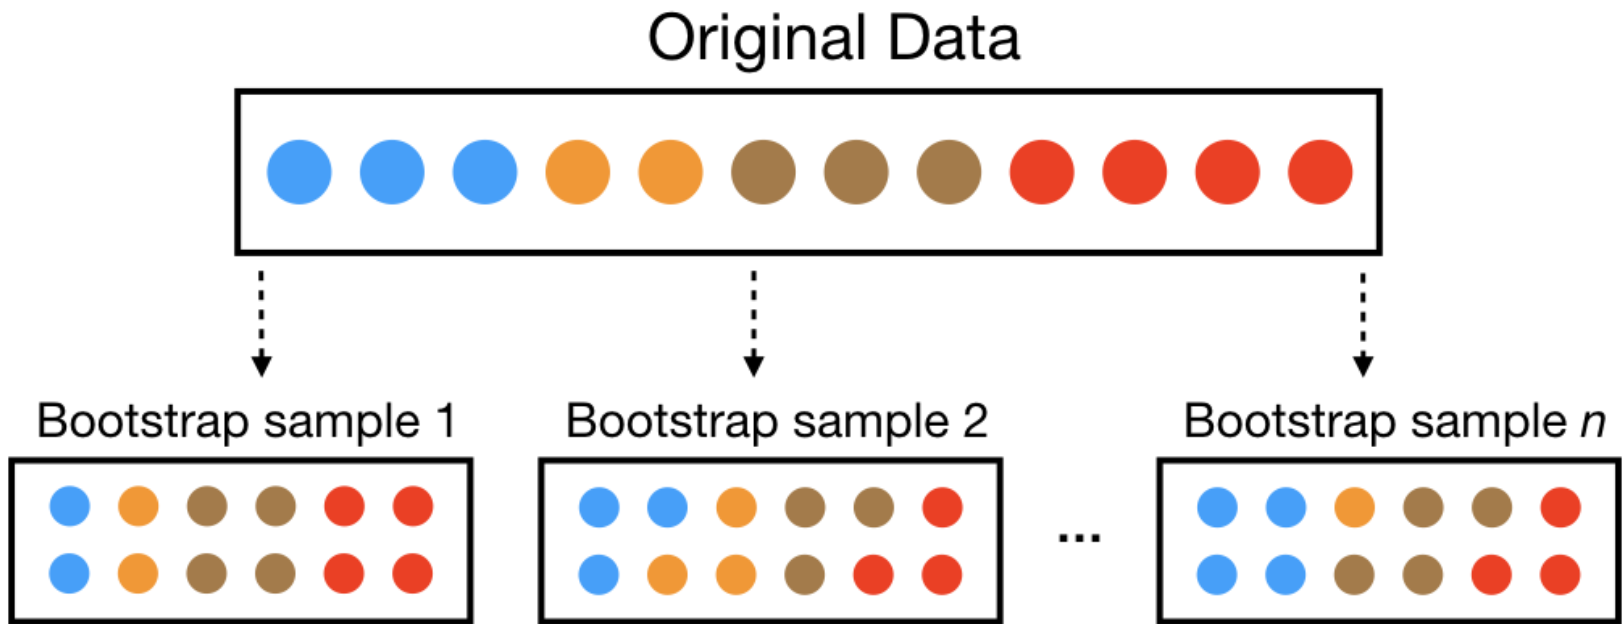
\includegraphics[width=1.0\textwidth]{figures/bootstrap_sampling.png}\\
		\href{https://datasciencedojo.com/blog/bootstrap-sampling/}{Source}
	\end{center}
\end{frame}

\frame{
    \frametitle{How does bagging work?}
    \begin{itemize}
        \item Create multiple bootstrap samples of the training data
        \item Train a base model (e.g.\ a decision tree) on each bootstrap sample
        \item Use each trained model to make predictions
        \item Combine predictions from all models (majority vote for classification or averaging for regression)
        \item Final prediction often has lower variance and improved generalization
        %COMMENT: Added explicit mention of classification vs regression voting scheme.
    \end{itemize}
}

\frame{
	\frametitle{Boosting}
	\begin{center}
		{\LARGE Boosting}
	\end{center}
}

\section{Boosting}
\frame{
    \frametitle{Boosting}
    \begin{itemize}
        \item A technique that combines multiple \emph{weak} learners sequentially
        \item Each subsequent model focuses more on samples that previous models misclassified (higher weight)
        \item Typically reduces bias, but can be prone to overfitting if not regularized
        \item Often uses simpler base learners (e.g.\ shallow trees), which are incrementally improved
        %COMMENT: Clarified that boosting is often used to reduce bias and that shallow base learners are common.
    \end{itemize}
}

\frame{
    \frametitle{How does boosting work?}
    \begin{enumerate}
        \item Initialize the weights of each training example equally
        \item Train a base model on the training data using the current weights
        \item Evaluate performance on the training data
        \item Increase weights of misclassified examples and decrease weights of correctly classified examples
        \item Repeat until stopping criterion (e.g.\ max iterations or minimal improvement)
        \item Final prediction is a weighted combination of all models' predictions
        \item \textbf{Learning rate} (\(\eta\)) often controls the contribution of each weak learner
        %COMMENT: Mentioned the learning rate as it is crucial for practical boosting algorithms.
    \end{enumerate}
}

\frame{
    \frametitle{AdaBoost and XGBoost}
    \begin{itemize}
        \item \textbf{AdaBoost}: Adaptive Boosting --- one of the earliest boosting algorithms
        \item \textbf{XGBoost}: eXtreme Gradient Boosting --- a popular gradient boosting framework
        \item Both typically use decision trees as base learners, though different objective and optimization strategies
        \item Widely used for tasks like image classification, ranking, and structured data problems
        %COMMENT: Clarified how AdaBoost and XGBoost fit into the boosting family.
    \end{itemize}
}

\frame{
    \frametitle{XGBoost features}
    \begin{enumerate}
        \item \textbf{Regularization}: includes L1 and L2 terms to prevent overfitting
        \item \textbf{Tree pruning}: prunes during construction to improve generalization
        \item \textbf{Handling missing values}: a built-in mechanism
        \item \textbf{Cross-validation}: integrated for hyperparameter tuning
        \item \textbf{Parallelization and out-of-core computation}: allows XGBoost to scale efficiently
        %COMMENT: Added mention of parallelization and out-of-core to highlight practical advantage of XGBoost.
    \end{enumerate}
}

\frame{
    \frametitle{Recap: Decision trees}
    \begin{itemize}
        \item Built by recursively splitting data into subsets based on a feature threshold that provides the best information gain
        \item Leaf nodes contain final predictions (class labels or numeric values)
        \item Advantages: easy to interpret, handle mixed data types, minimal preprocessing
        \item Disadvantages: prone to overfitting if unpruned, can be unstable w.r.t.\ small data changes
        %COMMENT: Added notes on advantages and disadvantages and minimal data preprocessing.
    \end{itemize}
}

\frame{
    \frametitle{Visualization of decision trees}

    \href{https://github.com/parrt/dtreeviz}{https://github.com/parrt/dtreeviz}

    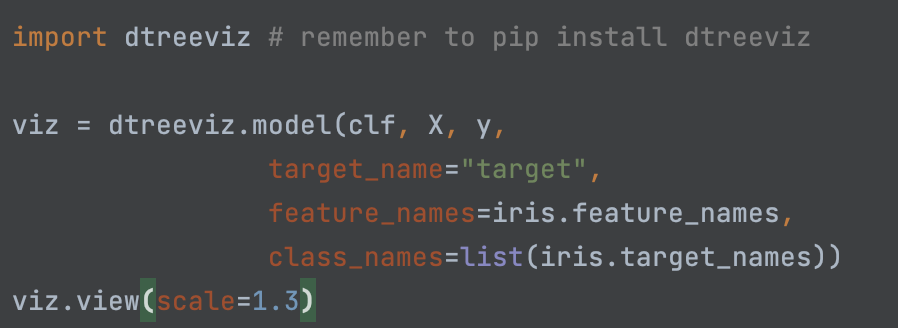
\includegraphics[width=0.8\textwidth]{figures/code_dttreeviz.png}
}

\frame{
    \frametitle{Visualization of decision trees}

    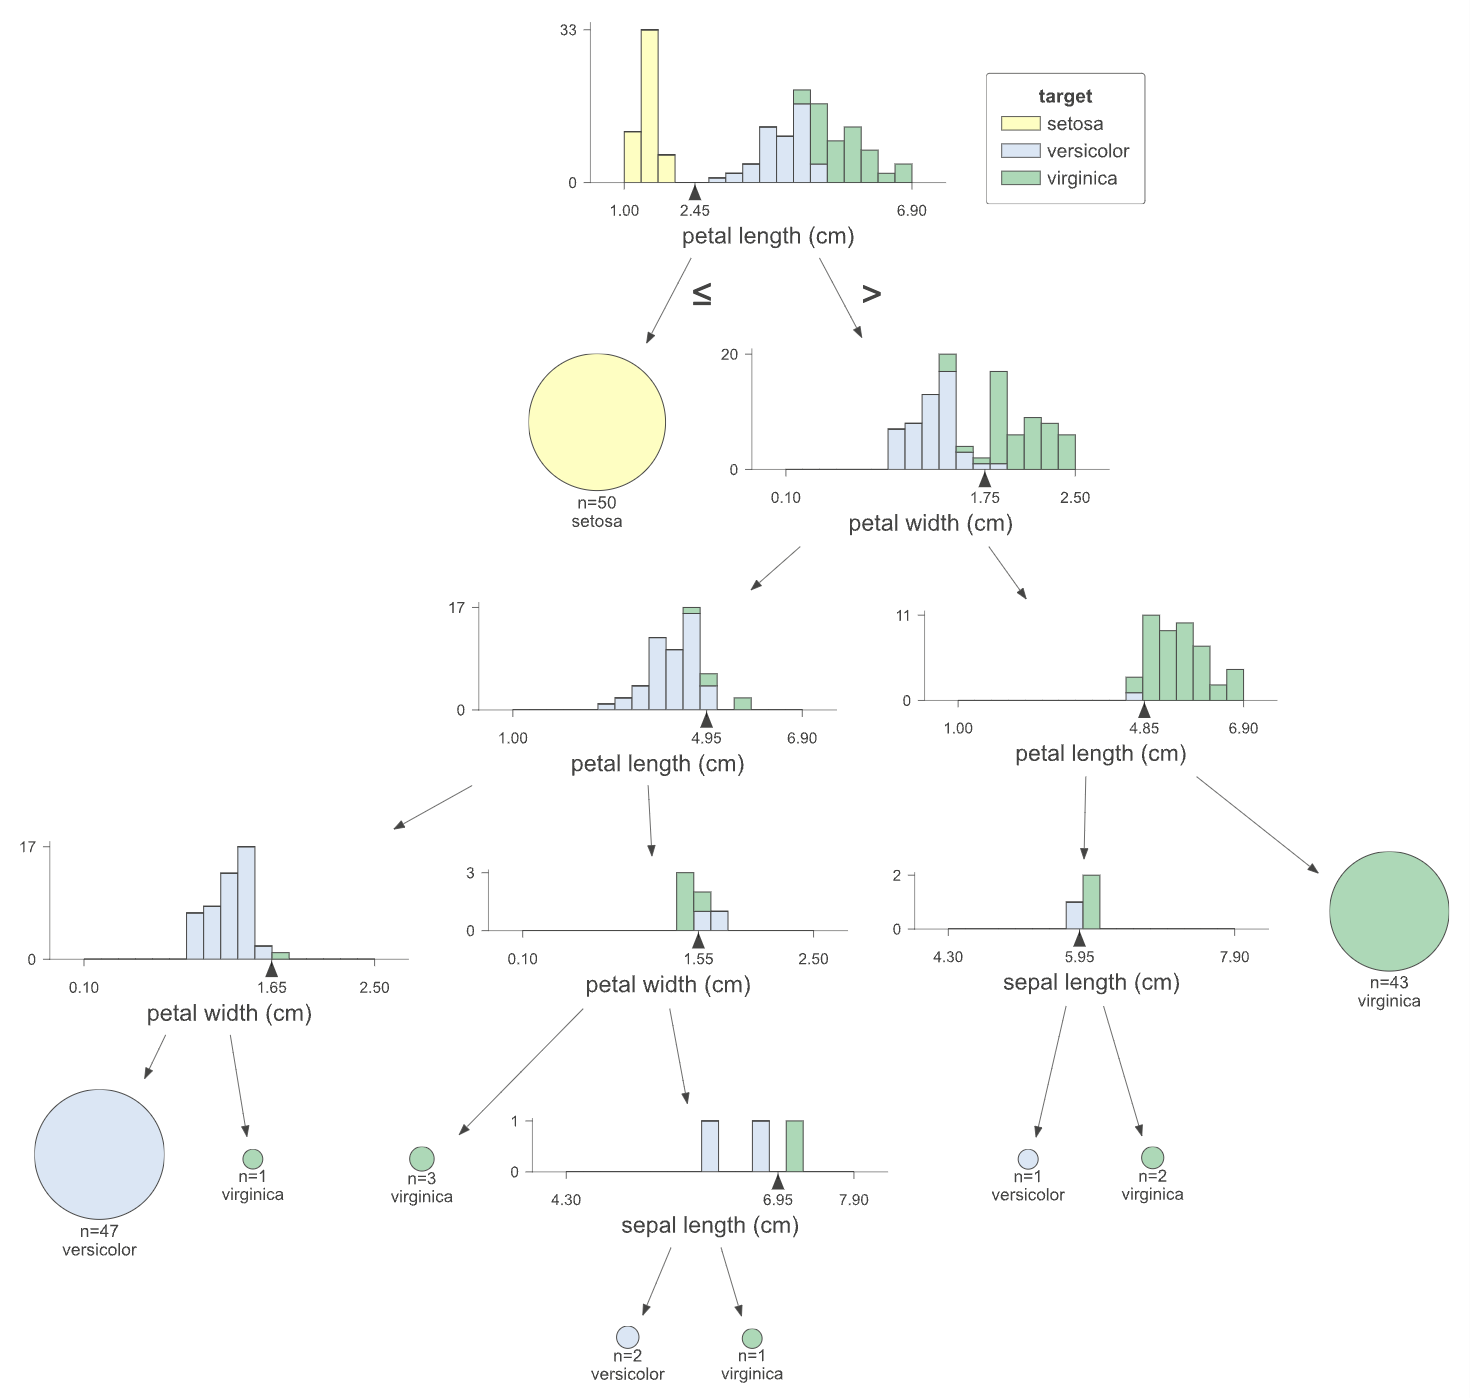
\includegraphics[width=0.5\textwidth]{figures/decision_tree.png}
}

\frame{
    \frametitle{Decision trees $\rightarrow$ Random forests}
    \begin{itemize}
        \item Bagging multiple decision trees alone can lead to highly correlated trees
        \item Random Forest adds \textbf{feature randomness} to reduce correlation among trees
        \item In addition to bootstrapping samples, each split considers only a random subset of features
        \item Reduces variance by decorrelating trees; improves predictive performance
        %COMMENT: Emphasized that random forests reduce correlation among trees, leading to better overall performance.
    \end{itemize}
}

\frame{
    \frametitle{De-correlated trees}
    \begin{enumerate}
        \item Each tree is built from a bootstrapped subset of the training data
        \item At each split, randomly select a set of predictors (e.g.\ \(\sqrt{p}\)) out of \(p\)
        \item From these predictors, choose the best predictor and threshold
        \item Result: lower correlation among trees and often higher accuracy
        %COMMENT: Added a clarifying final bullet on why lower correlation helps.
    \end{enumerate}
}

\frame{
    \frametitle{Random forests}
    \begin{itemize}
        \item Each decision tree in the ensemble is trained on a unique bootstrap sample
        \item Within each tree, only a subset of features is considered for splits
        \item Final classification prediction by majority vote; for regression, often averaged
        \item Provides good performance out-of-the-box and can handle large feature spaces
        %COMMENT: Added a note about majority vote vs. averaging and large feature spaces.
    \end{itemize}
}

\frame{
    \frametitle{Hyper-parameters for random forests}
    \begin{itemize}
        \item \texttt{n\_estimators}: number of trees. More trees can improve performance, but increases computation
        \item \texttt{max\_features}: number of features to consider at each split (often \(\sqrt{\text{number of features}}\))
        \item \texttt{max\_depth}: maximum depth of each tree. Deeper trees can overfit if not regularized
        \item \texttt{min\_samples\_split}: min number of samples required to further split a node
        \item \texttt{min\_samples\_leaf}: min number of samples in each leaf node
        \item Typically, random forests are quite robust to hyperparameter choices
        %COMMENT: Added a concluding statement about the robustness of RF to hyperparameters.
    \end{itemize}
}

\frame{
    \frametitle{Extra trees}
    \begin{itemize}
        \item Stands for \textbf{Extremely Randomized Trees}
        \item Similar to Random Forest in that multiple trees are trained on bootstrap samples
        \item At each node, a random subset of features is chosen (like in RF)
        \item \textbf{Key difference}: Extra Trees picks \textit{random} splitting thresholds, rather than searching for the optimal threshold
        \item This extra randomness can further reduce variance (but sometimes increases bias)
        %COMMENT: Clarified that Extra Trees uses random thresholds rather than the best threshold among all possible splits.
    \end{itemize}
}

\end{document}
